\subsection{Tūrinių ir poligoninių objektų palyginimas}

Gali susidaryti įspūdis, kad vokseliai realaus laiko kompiuterinėje grafikoje
tiesiogiai konkuruoja su poligonais. Gal taip ir buvo praeityje, bet dabar to
nėra, o ir ateityje mažai tikėtina, kad tas pasikartos -- greičiau jau išvysime
šių dviejų (ir kelių kitų) vizualizavimo koncepcijų susiliejimą ir bendrą
naudojimą, nei kad kuri nors iš jų dominuos, o kitos liks užmarštyje.

\subsubsection{Tūriniai objektai}

\begin{figure}[!ht]
\centering
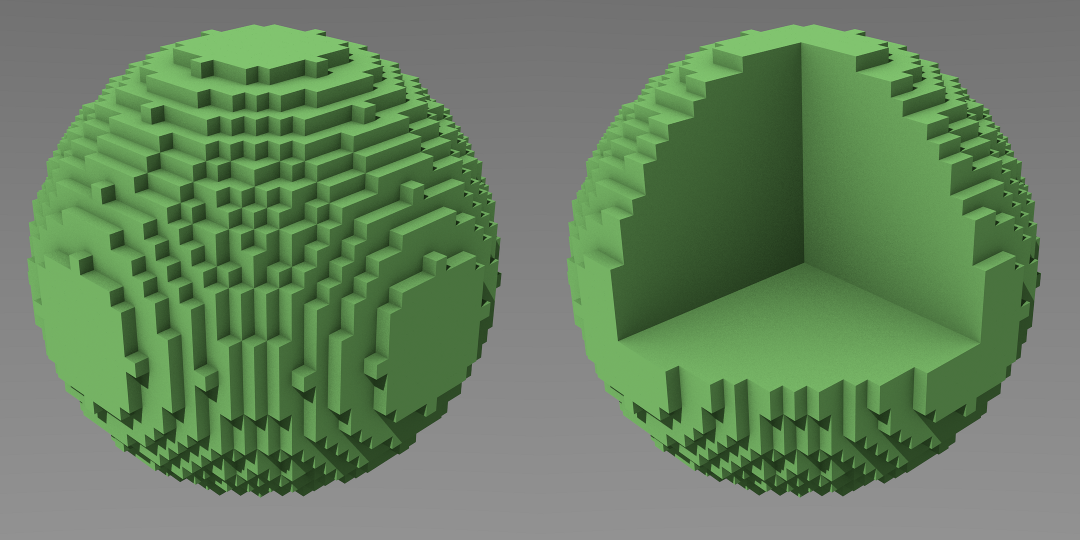
\includegraphics[width=16.5cm]{voxel_sphere.png}
\caption{Sfera, sudaryta iš vokselių. Pastaba: iliustraciniais tikslais
pasirinktas mažas detalumo lygmuo ir vizualizuojant nepritaikytos jokios
kampuotumą išlyginančios metodikos.}
\label{fig:voxel_sphere}
\end{figure}

Pliusai:

\begin{itemize}
\item Tūris
\item Detalumas
\item Pusiau permatomų objektų tikroviškumas
\item Paprastesnė duomenų struktūra
\end{itemize}

Minusai:

\begin{itemize}
\item Reikalauja daug atminties
\item Sudėtingas deformuojančio (Pavyzdžiui: kaulinė) animacijos įgyvendinimas
\item Aparatūrinės įrangos palaikymo nebuvimas
\item Mažas tūrinių objektų kūrimo įrankių pasirinkimas
\end{itemize}

\subsubsection{Poligonai objektai}

\begin{figure}[!ht]
\centering
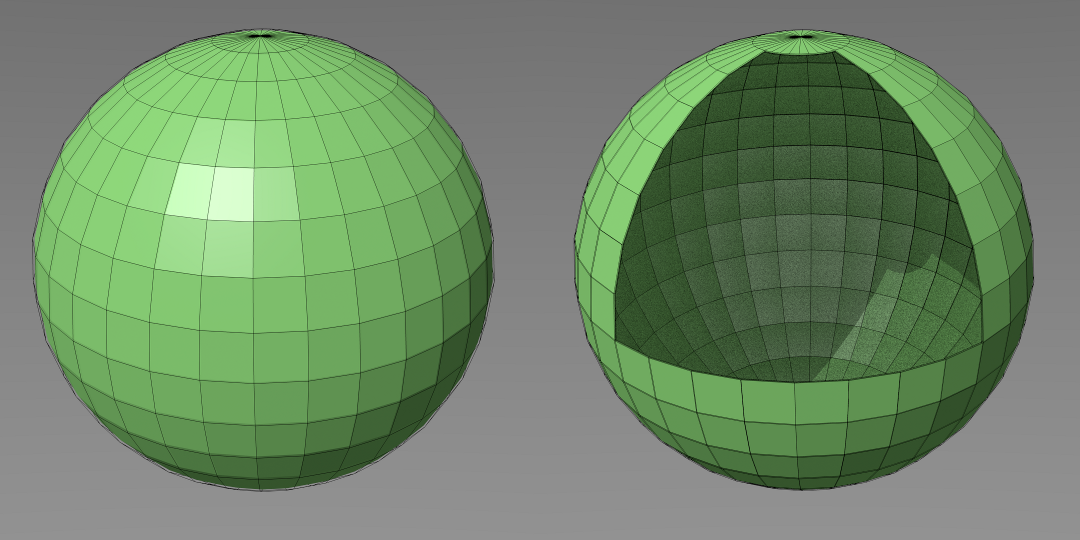
\includegraphics[width=16.5cm]{poly_sphere.png}
\caption{Sfera, iš poligonų. Atkreipkite dėmesį, kad ji tuščiavidurė.}
\label{fig:poly_sphere}
\end{figure}

Pliusai:

\begin{itemize}
\item Reikalauja mažiau atminties
\item Ganėtinai gerai prisitaiko prie deformuojančios animacijos
\item Gausybė kūrimo įrankių
\item Aparatūrinės įrangos palaikymas
\end{itemize}

Minusai:

\begin{itemize}
\item Prastokai susidoroja su pusiau permatomų objektų perteikimu
\item Sudėtingesnė duomenų struktūra
\item Tuščiaviduriai objektai
\end{itemize}

Tai nėra labai nuodugnus palyginimas, tačiau iš jo gana akivaizdu, kad
kiekviena koncepcija turi savo panaudojimo situacijas.

Pavyzdžiui: reikia vizualizuoti žmogaus kūną, kuris atliks įvairius judesius.
Ypatybės: nepermatomas objektas; deformuojančios animacijos. Pasirinkimas:
poligonai.

Reikia pavaizduoti dūmus. Ypatybės: pusiau permatomas tūrinis objektas;
dalelyčių animacija. Pasirinkimas: vokseliai.

Reikia pavaizduoti siena. Pasirinkimas: poligonai. Tą sieną bus galima
naikinti realiu laiku (tarkim betono siena, kurią galima išsprogdinti
dalimis). Tuomet pasirinkimas: vokseliai.

Akivaizdu, kad niekas netrukdo integruoti šias abi koncepcijas viena į kitą.
Pavyzdžiui: poligoninis nepermatomas žmogus formuoja vokselinę ledo skulptūrą.
Jis ne tik keičia skulptūros formą, bet ir pridaro joje daug skylių.

